\section{The Reasoning}
\label{sec::reasoning}

With all the different events laid out a deeper analysis of why those happened is now feasible. The reasons had to be major to justify how it started from nothing and went to become this new overwhelming force in the world of gaming.\\

But perhaps what could be more interesting is how the nature of those reasons that led Quake to its top position in the year 2000 quickly turned on it and ceased to be relevant given how the community had evolved and the new games that came to take Quake's spot at the zenith.\\

\subsection{Design: Skill-based Masterpiece}

A perfect example of what Caillois defined as a game of \textit{Agon} \citep{caillois1961man}, the game was quickly categorized as a skill-dependant game which required a ton of effort to perform. The next few paragraphs will focus on how it ended up being that way and, when applicable, why those design decision, mechanics or reasons are not compelling anymore.

\subsubsection{Unintended but Important}

Kicking things off on a light note there are the unplanned mechanics and the features the game had which created completely unforeseen situations.\\

\textbf{Strafe-Jumping} was a movement technique in Quake that allowed the player to jump in a certain way increasing his velocity past the theoretical programmed limit. If players chained together these jumps while achieving incredible speeds they would be using what was called \textbf{Bunny-Hopping}.\\

Both of those features were \textbf{completely unintended} and came from a bug in the movement related code yet they became so deeply important that the developers left said bug intact. The significance of \textbf{the mechanic was very relevant to the deeply competitive community}. It had a great impact on performance while being very hard to learn and master \parencite{speedRun}. Rocket-Jumping\footnote{Rocket-Jumping is a technique in which the player shoots a rocket near its feet while jumping to boost their speed and height} is another example of this.\\

But mechanics were not the only unintended but important aspect of the game. The developers fantasized at one point about having big \textbf{groups and clans} of people competing in their game but they themselves \textbf{did not expect} that to materialize nor they intended to make it happen \citep{clanHistory}. As we now know, it did in fact happen and it was what kicked things off as far as the first small eSports tournaments.

\subsubsection{Elitism, prowess and expertise}



\begin{figure}
	\begin{center}
		\fbox{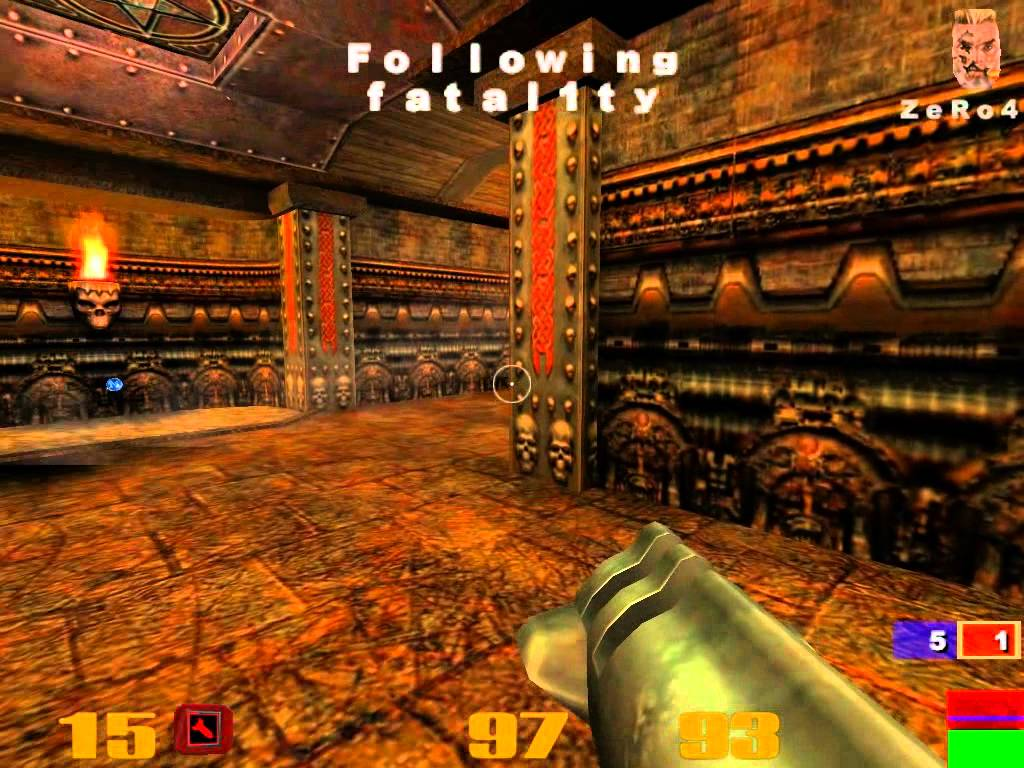
\includegraphics[width=0.95\linewidth]{resources/screenshot.jpg}}
		\caption{Competitive Screenshot. Captured from \href{https://www.youtube.com/watch?v=ka-5hEcU01k}{"Fatal1ty" vs "ZeRo4" on \nolinkurl{youtube.com}}}
	\end{center}
\end{figure}

The \textbf{main defining factor for Quake} which still applies today. The game had and still has an incredibly \textbf{high skill ceiling} and \textbf{massively steep learning curve} caused by the very \textbf{hard to learn mechanics}, \textbf{aim and movement focused gameplay} and the use of mainly the \textbf{1v1 mode} in the competitive scene.\\

In the \textbf{late 90s}, those factors were very appealing given the potential audience. In a time where competitive gaming was so small, the only \textbf{members of the community} were ones that now would be defined as "\textit{\textbf{hardcore gamers}}" or the "\textit{tryhards}". The core of the competitive gaming community found a game that focused on pure skill captivating.\\

But \textbf{the more a medium grows the more of its fan-base is composed of casual followers} instead of devoted aficionados. Such often called "\textit{casuals}" in a derogatory manner by the "\textit{hardcores}" are not as interested in getting into a game that required months or even years of practice to be able to grasp its mechanics and be a contestant.\\

Currently, a \textbf{main focus of massive competitive games is to give that fun, fast and forgiving experience} to the casual players, allowing them to amass colossal fan-bases that feed the eSports machine.\\

Quake could not be more different. The aim, movement, strategy focused gameplay and the general difficulty create this situation in which even a game with two very evenly matched players often ends in utter and complete domination. A \textbf{hugely unbalanced final score} in this game does not mean that one player is significantly better, the \textbf{skill gap might actually be minimal}. Conversely, imagine how \textbf{crushing} games can be to a new casual player who tries to compete with an old Quake veteran, the \textbf{experience would be demolishing}.\\

\begin{figure}
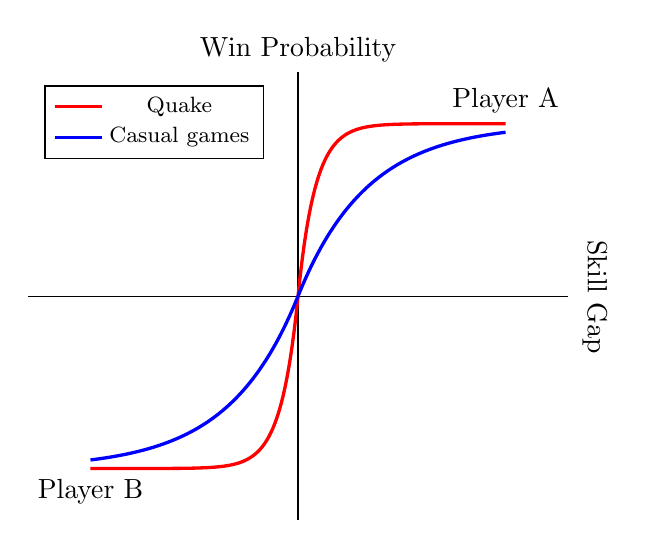
\begin{tikzpicture}
  	\begin{axis}[
  		legend pos=north west,
  		legend style = {font=\footnotesize},
		xmin=-1.3,xmax=1.3,
		ymin=-1.3,ymax=1.3,
		axis lines=center,
		axis line style=-,
		ticks=none,
		%y axis line style= { draw opacity=0 },
		%xticklabels={,,}
		x label style={at={(axis description cs:1.05,0.35)},anchor=east,rotate=270},
		y label style={at={(axis description cs:0.5,1.1)},anchor=north},
		xlabel={Skill Gap},
		ylabel={Win Probability}]
		domain=-1:1]
		\legend{Quake, Casual games}
		\addplot[-,red, very thick] expression[domain=0:1, samples=100]{ 	(1-e^(-12*x))		} node[color=black,above,pos=1] {Player A}; 
		\addplot[-,blue,very thick] expression[domain=0:1, samples=100]{ 	(1-e^(-3*x))		}; 
		\addplot[-,red, very thick] expression[domain=-1:0, samples=100]{	(e^(12*x))-1		} node[color=black,below,pos=0] {Player B}; 
		\addplot[-,blue,very thick] expression[domain=-1:0, samples=100]{	(e^(3*x))-1			}; 
  	\end{axis}
\end{tikzpicture}
  	\caption{Skill Gap to Win Probability relation}
	\label{fig:skillwin}
\end{figure}

This is explained in \textbf{Figure \ref{fig:skillwin}} which co-relates the probability that one player might win to the difference in skill between them. Values to the \textbf{top or to the right} indicate \textbf{positive or advantageous values for Player A}, when considering values to the \textbf{bottom or left} they are \textbf{positive or advantageous for Player B}.\\

If the \textbf{Skill Gap (in the X-axis)} is on Player A's side in a casual game (blue line) he has indeed a higher \textbf{Probability of winning (in the Y-axis)} than losing but this probability is much higher in Quake than in some other casual game. The red line shows how even when minimal skill gaps, the win probability of the slightly better player spikes way faster in Quake compared to casual games. This creates the situation explained previously where very unbalanced scores are common among similarly-skilled players in Quake-like games while not as common elsewhere.\\

Some reasons for this have already been mentioned, such as the difficulty curve. But the fact that the biggest eSports titles are \textbf{team based} is not by chance \parencite[p.~12]{van2013video}. A team game naturally softens that spike we see in Figure \ref{fig:skillwin}'s red line. Having more people playing for a side adds more random elements that could help swing the game in favour of the team with a bad player. Such bad player in a skill-based 1v1 game is likely to lose many more games than in a team-based title.\\

There are more elements that matter, such as the \textbf{in-game random elements} of some competitive games. Card games being a good example of this. In \textit{Hearthstone} \citep{game:hs} a player can match up with a competitor more skilled than himself and still win because of inherently random factors such as having a deck that is very good against the opponent's, getting better cards each turn while the opponent gets bad ones or a ton of random effects that the cards in that game originate.\\

There is a \textbf{famous anecdote} within Quake forums in which a friend of an old Quake veteran went to his house and played the game for the first time while his friend finished some tasks. When said veteran came back the casual player had mixed feelings, he liked the mechanics but he asked the infamous question:

\begin{quote}
\begin{center}
\textit{\textbf{Why can't I compete?}}
\end{center}
\end{quote}

Although he understood that winning should not be plausible for him he could not wrap his head around being utterly dismantled while not being able to even get a single kill even when he, as a beginner, was playing against Quake veterans that had put thousands of hours into the game. \textbf{This exemplifies the elitism of Quake}. If you go into a game against the top Quake player in the world you are likely to not get a single kill, in that very same case in \textit{Counter-Strike} or \textit{League or Legends} your team or you might even kill him a few times or even get some wins or rounds.\\

Rolling the dice and splitting responsibilities help casual players enjoy a game before they are good at it. Competitive Quake follows a \textbf{completely opposite philosophy} with its lack of random elements, skill-based game-play and 1v1 mode.\\ 


\subsection{Technology: Engineering Gem}

Many breakthrough features represented quantum leaps in-game technology when \textit{Quake} was released. The recurring theme of reasons why \textit{Quake} was at the top becoming irrelevant after a few years comes back vigorous in this section.\\

Since \textit{Quake} was the first game to incorporate this technology with such level of quality, they were obviously regarded avant-garde and innovative. Time went by and other developers caught up, in part helped by the fact that the source code of Quake was and still is readily available \citep{git:id}.\\

Some of the main advantages deserving mention were:

\begin{itemize}
	\item \textbf{Real three-dimensional engine}: Allowing 3D movement and the possibility of looking up and down. This was very impressible for old \textit{Doom} players that were used to that camera's lack of verticality.
	\item \textbf{Engine advancements}: While the game was astonishing for that era it ran very fluently. This was caused by smart rendering design decisions such as \textbf{pre-calculate lights and shadows}, \textbf{sectioning the maps} to avoid computing not currently visible, using \textbf{hardware acceleration} and pre-process maps to reduce the complexity of their geometry.
	\item \textbf{Best Netcode to date}: Used a Server/Client model was a significant improvement over having to directly dial the modem of the other player. Using a server provided not only a much more consistent experience but also support for more players and a much more convenient way to set up competitions or friendly matches.
	\item \textbf{Ease of modding and creating content}: Modify the game's code and create maps was a very easy task compared to other games at the time. The engine had such a good structure, quality and readability that it was used as a base for a wide variety of other hugely important engines \parencite{engineFamily} and today it is still a staple in-game engine and networking teaching environments.
\end{itemize}

\subsection{Situational: Other Causes}

The \textbf{lack of similar games} was a strong point for Quake's success but there were also other reasons deserving of mention.\\

A plethora of people claimed that they \textbf{bought Quake only for the single-player} since \textit{Doom} was already a huge success years before. Then when they had already played Quake's single-player mode and discovered the multi-player it opened this door of opportunity to keep enjoying the game differently. The game was not marketed for the multi-player, and people did not feel like they were gambling and buying this "new thing", in their eyes \textbf{they were investing in a single-player game} from a company they already trusted.\\

Something that kept the game from still being successful going forward is \textbf{id Software's tendency to focus on the game they are making, release it and move on to the next one}. In the current state of eSports, continuous support from the developers is a key component to make a successful competitive game, this enables necessary patches, sponsored events and in-game eSports focused content.\\

Last but not least there is the \textbf{creativity aspect of the game}. Much of the game success depended on how the community made maps and mods to then run those on their own servers. This made it so the player base naturally moved to the most liked versions of the game while having a great deal to choose from. \textbf{Currently, developers exercise massive control} over the content and versions of their product, which\textbf{ keeps the community from splitting} and creates a \textbf{consistent experience} at the cost of \textbf{eliminating that degree of creativity}.
